\documentclass{standalone}
\usepackage{pgfplots}
\pgfplotsset{compat=1.18}
\usepgfplotslibrary{colorbrewer}
\pgfplotsset{cycle list/Set1-6}

\begin{document}

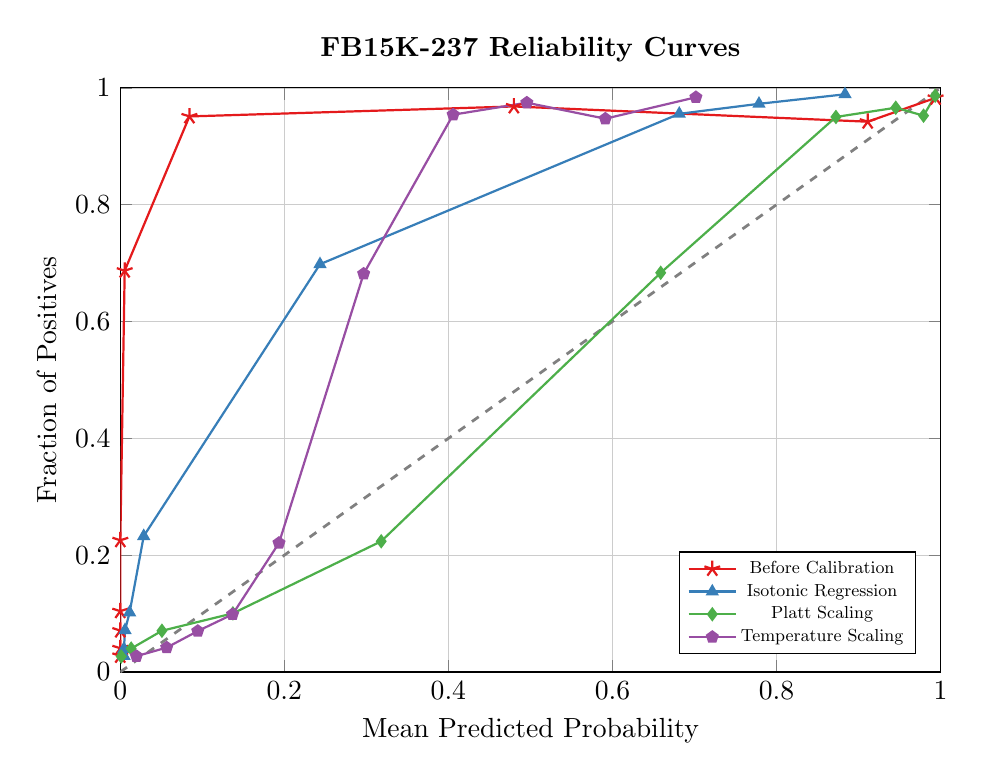
\begin{tikzpicture}
\begin{axis}[
    title={\textbf{FB15K-237 Reliability Curves}},
    xlabel={Mean Predicted Probability},
    ylabel={Fraction of Positives},
    xmin=0, xmax=1,
    ymin=0, ymax=1,
    xtick={0, 0.2, 0.4, 0.6, 0.8, 1.0},
    ytick={0, 0.2, 0.4, 0.6, 0.8, 1.0},
    legend pos= south east,
    legend style={nodes={scale=0.7, transform shape}, font=\small},
    grid=both,
    grid style={line width=.1pt, draw=gray!20},
    major grid style={line width=.2pt, draw=gray!40},
    width=12cm,
    height=9cm,
    cycle list name=Set1-6
]

% Perfectly Calibrated Line
\addplot [color=gray, dashed, line width=1pt, forget plot]
    coordinates {(0,0)(1,1)};

% Before Calibration (Baseline)
\addplot+[mark=star, thick, mark size=3pt] coordinates {
    (3.40e-11, 0.0276) (8.56e-09, 0.0406) (2.75e-07, 0.0709) (4.61e-06, 0.1041) (9.08e-05, 0.2255) (0.0054, 0.6870) (0.0843, 0.9511) (0.4798, 0.9682) (0.9111, 0.9421) (0.9939, 0.9829)
};
\addlegendentry{Before Calibration}

\addplot+[mark=triangle*, thick] coordinates {
    (0.0045, 0.0276) (0.0045, 0.0396) (0.0058, 0.0716) (0.0114, 0.1019) (0.0286, 0.2326) (0.2435, 0.6981) (0.6814, 0.9556) (0.7786, 0.9727) (0.8835, 0.9890)
};
\addlegendentry{Isotonic Regression}

\addplot+[mark=diamond*, thick] coordinates {
    (0.0012, 0.0266) (0.0133, 0.0401) (0.0508, 0.0706) (0.1373, 0.1004) (0.3181, 0.2238) (0.6588, 0.6834) (0.8724, 0.9502) (0.9453, 0.9660) (0.9792, 0.9524) (0.9934, 0.9866)
};
\addlegendentry{Platt Scaling}
\addplot+[mark=pentagon*, thick] coordinates {
    (0.0197, 0.0271) (0.0566, 0.0418) (0.0945, 0.0701) (0.1369, 0.0987) (0.1935, 0.2209) (0.2967, 0.6817) (0.4058, 0.9541) (0.4956, 0.9746) (0.5913, 0.9472) (0.7017, 0.9839)
};
\addlegendentry{Temperature Scaling}

\end{axis}
\end{tikzpicture}

\end{document}